% Options for packages loaded elsewhere
% Options for packages loaded elsewhere
\PassOptionsToPackage{unicode}{hyperref}
\PassOptionsToPackage{hyphens}{url}
%
\documentclass[
  ignorenonframetext,
  aspectratio=169,
  russian,
]{beamer}
\newif\ifbibliography
\usepackage{pgfpages}
\setbeamertemplate{caption}[numbered]
\setbeamertemplate{caption label separator}{: }
\setbeamercolor{caption name}{fg=normal text.fg}
\beamertemplatenavigationsymbolshorizontal
% remove section numbering
\setbeamertemplate{part page}{
  \centering
  \begin{beamercolorbox}[sep=16pt,center]{part title}
    \usebeamerfont{part title}\insertpart\par
  \end{beamercolorbox}
}
\setbeamertemplate{section page}{
  \centering
  \begin{beamercolorbox}[sep=12pt,center]{section title}
    \usebeamerfont{section title}\insertsection\par
  \end{beamercolorbox}
}
\setbeamertemplate{subsection page}{
  \centering
  \begin{beamercolorbox}[sep=8pt,center]{subsection title}
    \usebeamerfont{subsection title}\insertsubsection\par
  \end{beamercolorbox}
}
% Prevent slide breaks in the middle of a paragraph
\widowpenalties 1 10000
\raggedbottom
\AtBeginPart{
  \frame{\partpage}
}
\AtBeginSection{
  \ifbibliography
  \else
    \frame{\sectionpage}
  \fi
}
\AtBeginSubsection{
  \frame{\subsectionpage}
}
\usepackage{iftex}
\ifPDFTeX
  \usepackage[T1]{fontenc}
  \usepackage[utf8]{inputenc}
  \usepackage{textcomp} % provide euro and other symbols
\else % if luatex or xetex
  \usepackage{unicode-math} % this also loads fontspec
  \defaultfontfeatures{Scale=MatchLowercase}
  \defaultfontfeatures[\rmfamily]{Ligatures=TeX,Scale=1}
\fi
\usepackage{lmodern}

\ifPDFTeX\else
  % xetex/luatex font selection
\fi
% Use upquote if available, for straight quotes in verbatim environments
\IfFileExists{upquote.sty}{\usepackage{upquote}}{}
\IfFileExists{microtype.sty}{% use microtype if available
  \usepackage[]{microtype}
  \UseMicrotypeSet[protrusion]{basicmath} % disable protrusion for tt fonts
}{}

\usepackage{color}
\usepackage{fancyvrb}
\newcommand{\VerbBar}{|}
\newcommand{\VERB}{\Verb[commandchars=\\\{\}]}
\DefineVerbatimEnvironment{Highlighting}{Verbatim}{commandchars=\\\{\}}
% Add ',fontsize=\small' for more characters per line
\usepackage{framed}
\definecolor{shadecolor}{RGB}{241,243,245}
\newenvironment{Shaded}{\begin{snugshade}}{\end{snugshade}}
\newcommand{\AlertTok}[1]{\textcolor[rgb]{0.68,0.00,0.00}{#1}}
\newcommand{\AnnotationTok}[1]{\textcolor[rgb]{0.37,0.37,0.37}{#1}}
\newcommand{\AttributeTok}[1]{\textcolor[rgb]{0.40,0.45,0.13}{#1}}
\newcommand{\BaseNTok}[1]{\textcolor[rgb]{0.68,0.00,0.00}{#1}}
\newcommand{\BuiltInTok}[1]{\textcolor[rgb]{0.00,0.23,0.31}{#1}}
\newcommand{\CharTok}[1]{\textcolor[rgb]{0.13,0.47,0.30}{#1}}
\newcommand{\CommentTok}[1]{\textcolor[rgb]{0.37,0.37,0.37}{#1}}
\newcommand{\CommentVarTok}[1]{\textcolor[rgb]{0.37,0.37,0.37}{\textit{#1}}}
\newcommand{\ConstantTok}[1]{\textcolor[rgb]{0.56,0.35,0.01}{#1}}
\newcommand{\ControlFlowTok}[1]{\textcolor[rgb]{0.00,0.23,0.31}{\textbf{#1}}}
\newcommand{\DataTypeTok}[1]{\textcolor[rgb]{0.68,0.00,0.00}{#1}}
\newcommand{\DecValTok}[1]{\textcolor[rgb]{0.68,0.00,0.00}{#1}}
\newcommand{\DocumentationTok}[1]{\textcolor[rgb]{0.37,0.37,0.37}{\textit{#1}}}
\newcommand{\ErrorTok}[1]{\textcolor[rgb]{0.68,0.00,0.00}{#1}}
\newcommand{\ExtensionTok}[1]{\textcolor[rgb]{0.00,0.23,0.31}{#1}}
\newcommand{\FloatTok}[1]{\textcolor[rgb]{0.68,0.00,0.00}{#1}}
\newcommand{\FunctionTok}[1]{\textcolor[rgb]{0.28,0.35,0.67}{#1}}
\newcommand{\ImportTok}[1]{\textcolor[rgb]{0.00,0.46,0.62}{#1}}
\newcommand{\InformationTok}[1]{\textcolor[rgb]{0.37,0.37,0.37}{#1}}
\newcommand{\KeywordTok}[1]{\textcolor[rgb]{0.00,0.23,0.31}{\textbf{#1}}}
\newcommand{\NormalTok}[1]{\textcolor[rgb]{0.00,0.23,0.31}{#1}}
\newcommand{\OperatorTok}[1]{\textcolor[rgb]{0.37,0.37,0.37}{#1}}
\newcommand{\OtherTok}[1]{\textcolor[rgb]{0.00,0.23,0.31}{#1}}
\newcommand{\PreprocessorTok}[1]{\textcolor[rgb]{0.68,0.00,0.00}{#1}}
\newcommand{\RegionMarkerTok}[1]{\textcolor[rgb]{0.00,0.23,0.31}{#1}}
\newcommand{\SpecialCharTok}[1]{\textcolor[rgb]{0.37,0.37,0.37}{#1}}
\newcommand{\SpecialStringTok}[1]{\textcolor[rgb]{0.13,0.47,0.30}{#1}}
\newcommand{\StringTok}[1]{\textcolor[rgb]{0.13,0.47,0.30}{#1}}
\newcommand{\VariableTok}[1]{\textcolor[rgb]{0.07,0.07,0.07}{#1}}
\newcommand{\VerbatimStringTok}[1]{\textcolor[rgb]{0.13,0.47,0.30}{#1}}
\newcommand{\WarningTok}[1]{\textcolor[rgb]{0.37,0.37,0.37}{\textit{#1}}}

\usepackage{longtable,booktabs,array}
\newcounter{none} % for unnumbered tables
\usepackage{calc} % for calculating minipage widths
\usepackage{caption}
% Make caption package work with longtable
\makeatletter
\def\fnum@table{\tablename~\thetable}
\makeatother
\usepackage{graphicx}
\makeatletter
\newsavebox\pandoc@box
\newcommand*\pandocbounded[1]{% scales image to fit in text height/width
  \sbox\pandoc@box{#1}%
  \Gscale@div\@tempa{\textheight}{\dimexpr\ht\pandoc@box+\dp\pandoc@box\relax}%
  \Gscale@div\@tempb{\linewidth}{\wd\pandoc@box}%
  \ifdim\@tempb\p@<\@tempa\p@\let\@tempa\@tempb\fi% select the smaller of both
  \ifdim\@tempa\p@<\p@\scalebox{\@tempa}{\usebox\pandoc@box}%
  \else\usebox{\pandoc@box}%
  \fi%
}
% Set default figure placement to htbp
\def\fps@figure{htbp}
\makeatother



\ifLuaTeX
\usepackage[bidi=basic,shorthands=off,provide=*]{babel}
\else
\usepackage[bidi=default,shorthands=off,provide=*]{babel}
\fi
\ifLuaTeX
  \usepackage{selnolig} % disable illegal ligatures
\fi


\setlength{\emergencystretch}{3em} % prevent overfull lines

\providecommand{\tightlist}{%
  \setlength{\itemsep}{0pt}\setlength{\parskip}{0pt}}



 

\usepackage[]{csquotes}

\IfFileExists{plex-otf.sty}{
  %% Full TeXlive
  % \usepackage[%
  %   % math,
  %   RM={Scale=0.94},SS={Scale=0.94},SScon={Scale=0.94},TT={Scale=MatchLowercase,FakeStretch=0.9},DefaultFeatures={Ligatures=Common}
  % ]{plex-otf}
}{
  %% TinyTeX
  \usepackage{libertine}
}

%%% Load theme
% https://deic.uab.cat/~iblanes/beamer_gallery/
\IfFileExists{beamerthemegotham.sty}{
  %% Full TeXlive
  \usetheme{gotham}
  \gothamset{
    numbering=totalpagenumber,
    parttocframe default=off,
    sectiontocframe default=off,
    subsectiontocframe default=off,
  }
}{
  %% TinyTeX
  \usetheme{Madrid}
}
\makeatletter
\@ifpackageloaded{caption}{}{\usepackage{caption}}
\AtBeginDocument{%
\ifdefined\contentsname
  \renewcommand*\contentsname{Содержание}
\else
  \newcommand\contentsname{Содержание}
\fi
\ifdefined\listfigurename
  \renewcommand*\listfigurename{Список иллюстраций}
\else
  \newcommand\listfigurename{Список иллюстраций}
\fi
\ifdefined\listtablename
  \renewcommand*\listtablename{Список таблиц}
\else
  \newcommand\listtablename{Список таблиц}
\fi
\ifdefined\figurename
  \renewcommand*\figurename{Рисунок}
\else
  \newcommand\figurename{Рисунок}
\fi
\ifdefined\tablename
  \renewcommand*\tablename{Таблица}
\else
  \newcommand\tablename{Таблица}
\fi
}
\@ifpackageloaded{float}{}{\usepackage{float}}
\floatstyle{ruled}
\@ifundefined{c@chapter}{\newfloat{codelisting}{h}{lop}}{\newfloat{codelisting}{h}{lop}[chapter]}
\floatname{codelisting}{Список}
\newcommand*\listoflistings{\listof{codelisting}{Листинги}}
\makeatother
\makeatletter
\makeatother
\makeatletter
\@ifpackageloaded{caption}{}{\usepackage{caption}}
\@ifpackageloaded{subcaption}{}{\usepackage{subcaption}}
\makeatother

\usepackage{bookmark}
\IfFileExists{xurl.sty}{\usepackage{xurl}}{} % add URL line breaks if available
\urlstyle{same}
% fallback for those not using the hyperref driver hyperxmp:
\makeatletter
\@ifundefined{xmpquote}{\newcommand{\xmpquote}[1]{#1}}{}
\makeatother
\hypersetup{
  pdftitle={Лабораторная работа №6},
  pdfauthor={Кудякова София Андреевна},
  pdflang={ru},
  hidelinks,
  pdfcreator={LaTeX via pandoc}}


\title{\texorpdfstring{Лабораторная работа №6}{Лабораторная работа №6}}
\subtitle{\texorpdfstring{Реализация основных моделей в подходе сетей
Петри}{Реализация основных моделей в подходе сетей Петри}}
\author{Кудякова София Андреевна}
\date{2026-08-29}

\begin{document}
\frame{\titlepage}

\renewcommand*\contentsname{Содержание}
\begin{frame}[allowframebreaks]
  \frametitle{Содержание}
  \setcounter{tocdepth}{1}
  \tableofcontents
\end{frame}
\setcounter{tocdepth}{1}
\tableofcontents
}

\section{Цель
работы}\label{ux446ux435ux43bux44c-ux440ux430ux431ux43eux442ux44b}

\begin{frame}{Цель работы}
\begin{enumerate}[<+->]
\tightlist
\item
  Реализовать модель эпидемии SIR с помощью сетей Петри.
\item
  Провести детерминированную и стохастическую симуляции.
\item
  Исследовать влияние коэффициента заражения \(\beta\) на динамику
  эпидемии.
\item
  Создать анимацию эпидемического процесса.
\item
  Выполнить параметрическое исследование модели.
\item
  Преобразовать код в литературный стиль и создать производные форматы.
\end{enumerate}
\end{frame}

\section{Сеть
Петри}\label{ux441ux435ux442ux44c-ux43fux435ux442ux440ux438}

\begin{frame}{Сеть Петри}
Сеть Петри представляет собой математический аппарат для моделирования
дискретных систем.

Она состоит из:

\begin{itemize}[<+->]
\tightlist
\item
  позиций;
\item
  переходов;
\item
  дуг;
\item
  маркировки сети.
\end{itemize}

Позиции содержат фишки и описывают состояние системы, а переходы
соответствуют событиям, которые изменяют это состояние.

Формально сеть Петри задаётся:

\[
N=(P,T,F,M_0),
\]

где:

\begin{itemize}[<+->]
\tightlist
\item
  \(P\) --- множество позиций;
\item
  \(T\) --- множество переходов;
\item
  \(F\) --- множество дуг;
\item
  \(M_0\) --- начальная маркировка.
\end{itemize}
\end{frame}

\section{Модель SIR}\label{ux43cux43eux434ux435ux43bux44c-sir}

\begin{frame}{Модель SIR}
Модель SIR описывает распространение инфекции, разделяя население на три
группы:

\begin{itemize}[<+->]
\tightlist
\item
  \(S\) --- восприимчивые к заболеванию;
\item
  \(I\) --- инфицированные;
\item
  \(R\) --- выздоровевшие.
\end{itemize}

Суммарная численность населения сохраняется:

\[
S+I+R=N.
\]

Детерминированная модель описывается системой:

\[
\begin{aligned}
\frac{dS}{dt} &= -\beta SI, \\
\frac{dI}{dt} &= \beta SI-\gamma I, \\
\frac{dR}{dt} &= \gamma I.
\end{aligned}
\]

В работе использовалась начальная маркировка:

\[
S=990,\qquad I=10,\qquad R=0.
\]
\end{frame}

\section{SIR как сеть
Петри}\label{sir-ux43aux430ux43a-ux441ux435ux442ux44c-ux43fux435ux442ux440ux438}

\begin{frame}[fragile]{SIR как сеть Петри}
Модель SIR представляется двумя основными переходами.

\textbf{Заражение:}

\[
S+I\rightarrow I+I
\]

\textbf{Выздоровление:}

\[
I\rightarrow R
\]

Изменение количества фишек в позициях сети Петри соответствует изменению
численности восприимчивых, инфицированных и выздоровевших.

Для реализации используются:

\begin{itemize}[<+->]
\tightlist
\item
  \texttt{AlgebraicPetri};
\item
  \texttt{OrdinaryDiffEq};
\item
  алгоритм Гиллеспи.
\end{itemize}
\end{frame}

\section{Базовое
моделирование}\label{ux431ux430ux437ux43eux432ux43eux435-ux43cux43eux434ux435ux43bux438ux440ux43eux432ux430ux43dux438ux435}

\begin{frame}[fragile]{Базовое моделирование}
Для базового эксперимента использовались параметры:

\[
\beta=0.3,\qquad
\gamma=0.1,\qquad
T=100.
\]

Начальная маркировка:

\[
S=990,\qquad I=10,\qquad R=0.
\]

Скрипт \texttt{sirpetri\_run.jl} выполняет:

\begin{itemize}[<+->]
\tightlist
\item
  детерминированное моделирование;
\item
  стохастическое моделирование.
\end{itemize}

Результаты сохраняются в:

\begin{Shaded}
\begin{Highlighting}[]
\NormalTok{data/sir\_det.csv}
\NormalTok{data/sir\_stoch.csv}
\end{Highlighting}
\end{Shaded}
\end{frame}

\section{Детерминированная
динамика}\label{ux434ux435ux442ux435ux440ux43cux438ux43dux438ux440ux43eux432ux430ux43dux43dux430ux44f-ux434ux438ux43dux430ux43cux438ux43aux430}

\begin{frame}{Детерминированная динамика}
\begin{figure}

\centering{


\includegraphics[width=0.85\linewidth,height=\textheight,keepaspectratio]{image/1.png}

}

\caption{\label{fig-det}Динамика детерминированной модели SIR}

\end{figure}%

На графике наблюдается характерная эпидемическая динамика:

\begin{itemize}[<+->]
\tightlist
\item
  число восприимчивых уменьшается;
\item
  число инфицированных сначала возрастает;
\item
  количество инфицированных достигает максимума;
\item
  затем число инфицированных снижается;
\item
  количество выздоровевших увеличивается.
\end{itemize}
\end{frame}

\section{Стохастическая
динамика}\label{ux441ux442ux43eux445ux430ux441ux442ux438ux447ux435ux441ux43aux430ux44f-ux434ux438ux43dux430ux43cux438ux43aux430}

\begin{frame}{Стохастическая динамика}
\begin{figure}

\centering{


\includegraphics[width=0.85\linewidth,height=\textheight,keepaspectratio]{image/2.png}

}

\caption{\label{fig-stoch}Динамика стохастической модели SIR}

\end{figure}%

Стохастическая модель имеет аналогичную общую динамику.

При этом отдельные значения испытывают случайные флуктуации относительно
детерминированного поведения.
\end{frame}

\section{\texorpdfstring{Исследование влияния
\(\beta\)}{Исследование влияния \textbackslash beta}}\label{ux438ux441ux441ux43bux435ux434ux43eux432ux430ux43dux438ux435-ux432ux43bux438ux44fux43dux438ux44f-beta}

\begin{frame}[fragile]{Исследование влияния \(\beta\)}
Для исследования влияния коэффициента заражения использовался скрипт:

\begin{Shaded}
\begin{Highlighting}[]
\NormalTok{scripts/sirpetri\_scan\_parameters.jl}
\end{Highlighting}
\end{Shaded}

Была выполнена серия детерминированных экспериментов при различных
значениях \(\beta\) при фиксированной скорости выздоровления.

Результаты сохраняются в:

\begin{Shaded}
\begin{Highlighting}[]
\NormalTok{data/sir\_scan.csv}
\end{Highlighting}
\end{Shaded}
\end{frame}

\section{Влияние коэффициента
заражения}\label{ux432ux43bux438ux44fux43dux438ux435-ux43aux43eux44dux444ux444ux438ux446ux438ux435ux43dux442ux430-ux437ux430ux440ux430ux436ux435ux43dux438ux44f}

\begin{frame}{Влияние коэффициента заражения}
\begin{figure}

\centering{


\includegraphics[width=0.85\linewidth,height=\textheight,keepaspectratio]{image/3.png}

}

\caption{\label{fig-scan}Влияние коэффициента заражения β на динамику
эпидемии}

\end{figure}%

Полученный график показывает, что увеличение коэффициента \(\beta\)
приводит к более интенсивному распространению инфекции.

При увеличении \(\beta\):

\begin{itemize}[<+->]
\tightlist
\item
  инфекция распространяется быстрее;
\item
  возрастает максимальное число одновременно инфицированных;
\item
  увеличивается масштаб эпидемического процесса.
\end{itemize}
\end{frame}

\section{Анимация эпидемического
процесса}\label{ux430ux43dux438ux43cux430ux446ux438ux44f-ux44dux43fux438ux434ux435ux43cux438ux447ux435ux441ux43aux43eux433ux43e-ux43fux440ux43eux446ux435ux441ux441ux430}

\begin{frame}[fragile]{Анимация эпидемического процесса}
Для визуализации изменения состояния системы во времени использовался
скрипт:

\begin{Shaded}
\begin{Highlighting}[]
\NormalTok{scripts/sirpetri\_animate.jl}
\end{Highlighting}
\end{Shaded}

Результат сохраняется в:

\begin{Shaded}
\begin{Highlighting}[]
\NormalTok{plots/sir\_animation.gif}
\end{Highlighting}
\end{Shaded}

\begin{figure}

\centering{

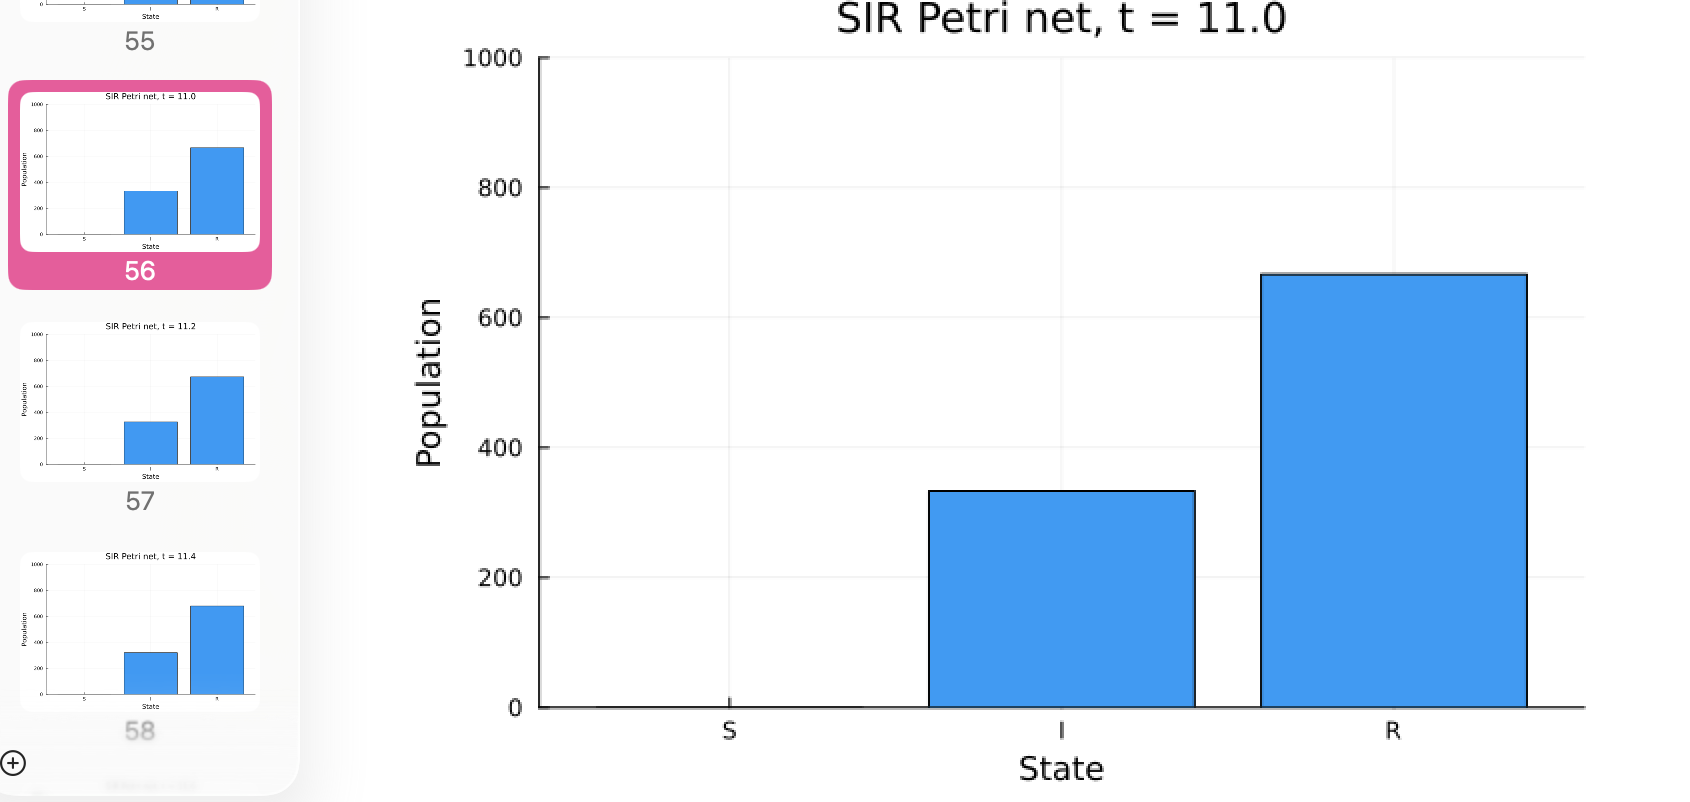
\includegraphics[width=0.75\linewidth,height=\textheight,keepaspectratio]{image/sir_animation.png}

}

\caption{\label{fig-animation}Кадр анимации динамики модели SIR}

\end{figure}%

Анимация позволяет наблюдать изменение трёх групп населения во времени:

\begin{itemize}[<+->]
\tightlist
\item
  уменьшение числа восприимчивых;
\item
  рост и последующее снижение числа инфицированных;
\item
  увеличение числа выздоровевших.
\end{itemize}
\end{frame}

\section{Сравнение
моделей}\label{ux441ux440ux430ux432ux43dux435ux43dux438ux435-ux43cux43eux434ux435ux43bux435ux439}

\begin{frame}[fragile]{Сравнение моделей}
Скрипт:

\begin{Shaded}
\begin{Highlighting}[]
\NormalTok{scripts/sirpetri\_report.jl}
\end{Highlighting}
\end{Shaded}

использует сохранённые результаты моделирования и формирует итоговые
графики.

\begin{figure}

\centering{


\includegraphics[width=0.85\linewidth,height=\textheight,keepaspectratio]{image/4.png}

}

\caption{\label{fig-comparison}Сравнение детерминированной и
стохастической моделей SIR}

\end{figure}%

Детерминированная модель задаёт гладкую траекторию.

Стохастическая модель содержит случайные отклонения, однако сохраняет
общий характер эпидемической динамики.
\end{frame}

\section{\texorpdfstring{Чувствительность к
\(\beta\)}{Чувствительность к \textbackslash beta}}\label{ux447ux443ux432ux441ux442ux432ux438ux442ux435ux43bux44cux43dux43eux441ux442ux44c-ux43a-beta}

\begin{frame}{Чувствительность к \(\beta\)}
\begin{figure}

\centering{


\includegraphics[width=0.85\linewidth,height=\textheight,keepaspectratio]{image/5.png}

}

\caption{\label{fig-sensitivity}Чувствительность максимального числа
инфицированных к коэффициенту β}

\end{figure}%

Рост \(\beta\) приводит к увеличению интенсивности эпидемического
процесса и изменению максимального числа инфицированных.

Таким образом, модель чувствительна к коэффициенту заражения.
\end{frame}

\section{Параметрическое
исследование}\label{ux43fux430ux440ux430ux43cux435ux442ux440ux438ux447ux435ux441ux43aux43eux435-ux438ux441ux441ux43bux435ux434ux43eux432ux430ux43dux438ux435}

\begin{frame}[fragile]{Параметрическое исследование}
Для дополнительного исследования использовался скрипт:

\begin{Shaded}
\begin{Highlighting}[]
\NormalTok{scripts/parameterized.jl}
\end{Highlighting}
\end{Shaded}

Он позволяет выполнять моделирование для различных наборов параметров
модели.

Результаты параметрического исследования представлены в:

\begin{Shaded}
\begin{Highlighting}[]
\NormalTok{notebooks/parameterized.ipynb}
\end{Highlighting}
\end{Shaded}

\begin{figure}

\centering{


\includegraphics[width=0.85\linewidth,height=\textheight,keepaspectratio]{image/7.png}

}

\caption{\label{fig-parameterized}Результат выполнения
параметризованного эксперимента в Jupyter Notebook}

\end{figure}%

Параметризация позволяет:

\begin{itemize}[<+->]
\tightlist
\item
  изменять исходные параметры модели;
\item
  выполнять серию экспериментов;
\item
  сравнивать результаты;
\item
  воспроизводить вычислительный эксперимент.
\end{itemize}
\end{frame}

\section{Литературное
программирование}\label{ux43bux438ux442ux435ux440ux430ux442ux443ux440ux43dux43eux435-ux43fux440ux43eux433ux440ux430ux43cux43cux438ux440ux43eux432ux430ux43dux438ux435}

\begin{frame}[fragile]{Литературное программирование}
Для оформления исходного кода в литературном стиле был создан файл:

\begin{Shaded}
\begin{Highlighting}[]
\NormalTok{scripts/sirpetri\_literate.jl}
\end{Highlighting}
\end{Shaded}

Литературное программирование объединяет программный код с поясняющим
текстом.

В результате были сформированы:

\begin{Shaded}
\begin{Highlighting}[]
\NormalTok{notebooks/sirpetri\_literate.ipynb}
\NormalTok{report/sirpetri\_literate.qmd}
\NormalTok{report/parameterized.qmd}
\end{Highlighting}
\end{Shaded}

Такой подход позволяет одновременно представить алгоритм, его описание и
результаты вычислений.
\end{frame}

\section{Структура
проекта}\label{ux441ux442ux440ux443ux43aux442ux443ux440ux430-ux43fux440ux43eux435ux43aux442ux430}

\begin{frame}[fragile]{Структура проекта}
Основная структура проекта:

\begin{Shaded}
\begin{Highlighting}[]
\NormalTok{project/}
\NormalTok{├── data/}
\NormalTok{│   ├── sir\_det.csv}
\NormalTok{│   ├── sir\_scan.csv}
\NormalTok{│   └── sir\_stoch.csv}
\NormalTok{├── notebooks/}
\NormalTok{│   ├── parameterized.ipynb}
\NormalTok{│   └── sirpetri\_literate.ipynb}
\NormalTok{├── plots/}
\NormalTok{│   ├── comparison.png}
\NormalTok{│   ├── sensitivity.png}
\NormalTok{│   ├── sir\_animation.gif}
\NormalTok{│   ├── sir\_det\_dynamics.png}
\NormalTok{│   ├── sir\_scan.png}
\NormalTok{│   └── sir\_stoch\_dynamics.png}
\NormalTok{├── report/}
\NormalTok{│   ├── parameterized.qmd}
\NormalTok{│   └── sirpetri\_literate.qmd}
\NormalTok{├── scripts/}
\NormalTok{│   ├── parameterized.jl}
\NormalTok{│   ├── sirpetri\_animate.jl}
\NormalTok{│   ├── sirpetri\_literate.jl}
\NormalTok{│   ├── sirpetri\_report.jl}
\NormalTok{│   ├── sirpetri\_run.jl}
\NormalTok{│   └── sirpetri\_scan\_parameters.jl}
\NormalTok{└── src/}
\NormalTok{    └── SIRPetri.jl}
\end{Highlighting}
\end{Shaded}

Такая структура разделяет:

\begin{itemize}[<+->]
\tightlist
\item
  исходный код;
\item
  данные;
\item
  результаты моделирования;
\item
  документацию;
\item
  Jupyter-ноутбуки.
\end{itemize}
\end{frame}

\section{Основные
результаты}\label{ux43eux441ux43dux43eux432ux43dux44bux435-ux440ux435ux437ux443ux43bux44cux442ux430ux442ux44b}

\begin{frame}{Основные результаты}
В ходе работы:

\begin{itemize}[<+->]
\tightlist
\item
  реализована модель SIR на основе сети Петри;
\item
  выполнено детерминированное моделирование;
\item
  выполнено стохастическое моделирование;
\item
  исследовано влияние \(\beta\);
\item
  построены графики динамики;
\item
  создана анимация;
\item
  выполнено сравнение моделей;
\item
  проведено параметрическое исследование;
\item
  реализовано литературное программирование;
\item
  созданы Jupyter-ноутбуки и Quarto-документы.
\end{itemize}
\end{frame}

\section{Выводы}\label{ux432ux44bux432ux43eux434ux44b}

\begin{frame}{Выводы}
Сети Петри позволяют удобно представлять переходы между состояниями
эпидемиологической модели.

Детерминированная и стохастическая модели демонстрируют общий характер
распространения инфекции, однако стохастическая модель дополнительно
учитывает случайные отклонения.

Изменение коэффициента \(\beta\) существенно влияет на скорость и
масштаб распространения инфекции.

Параметрическое исследование позволяет воспроизводимо изучать поведение
модели при различных исходных условиях.

Литературное программирование объединяет исходный код, пояснения и
результаты вычислений в едином представлении.
\end{frame}




\end{document}
